\documentclass[12pt]{article}
\usepackage{graphicx}
\usepackage{amsmath,amssymb}
\usepackage{caption}
\usepackage{hyperref}
\textheight 240mm
\textwidth  170mm
\oddsidemargin  0mm
\evensidemargin 0mm
\topmargin -20mm
\begin{document}
%_________________________________________________________________
\title{Automated Music Genre Classification}
\author{James Folberth, Dale Jennings, Alyson Fox}
\date{15 December, 2014}
\maketitle
%_________________________________________________________________
\section{Introduction}
%_________________________________________________________________
\indent Digital music has changed the face of music collection. Users can have a megabyte or a gigabyte worth of music on their personal laptops and can easily download music from the internet. This has lead to the need to invent and test new tools in musical information retrieval. There are many websites and apps, Pandora and iTunes are a few examples, that can create playlists based on similarity to a certain song or genre of music. These sites need to be able to classify certain features of a song and build the playlist from there.\\

The goal of this project is to able to classify the genre of a song. This may seem like a simple problem, since we can usually classify a song by ear, but that relies on the user having a vast knowledge of music. If we can automate the process using computers, we could find new and interesting insights that may not be obvious. However, this adds complexity that must be dealt with since we need techniques so that  the computer can ``listen'' to the song and extract features to be able to identify the genre. To do this we take  a song, which is a continuous signal and we sample at certain frequency to transform it into a discrete signal that is based on pitch which created by the sound pressures changes  and define it as a function of time. From the discrete signal we can define  ``features" for each song that may be able to be used to classify the genre.\\

 For our project we are only classifying within six different genres: classical, electronic, jazz/blues, metal/punk, rock/pop, and world. To compute similarities between each song it is imperative that we generate features. Given 729 training tracks, we will construct features for each song and the song that we would like to classify. We can use theses quantifiable features to develop a machine learning algorithm to classify the genre. Most features that we used were developed by or used in Elias Pampalk dissertation \cite{pampalk:dissertation} or in Tzanetakis and Cook \cite{tzanetakis:classification}.

%_________________________________________________________________
\section{Distance in song-space}
% TODO Dale's going to clean this up.

When trying to define a distance in song-space for genre classification, it is not very helpful to try to construct a distance based solely on the raw data.  Instead, feature extraction is applied to the songs in an attempt to represent each song in a manner that is more similar to how the human ear and brain perceives songs.  Having this quantification of musical features allows songs to be classified in a manner more similar to how a human might classify the songs.

\subsection{Preprocessing}

The first step in feature extraction is in preprocessing the song, where the raw pulse code modulation form of the song is transformed into segments of spectral information.  The preprocessing improves the accessibility of the features and is also the first step in dimensionality reduction.

\subsubsection{Power Spectrum}
The power spectrum of an audio signal is a frequency-domain representation of the signal.  More specifically, we use a short-time Fourier transform to transform the signal to the frequency-domain, while maintaining some temporal locality.  The signal is broken up into many small, possibly overlapping segments, each of which then is windowed and passed through a Fourier transform.  Once in the frequency domain, the square magnitude is calculated, to get the power spectrum.

\subsubsection{Mel Frequency Cepstrum}
While the power spectrum of a signal presents some nice information of the signal, the human ear processes audio signals in a different manner.  The Mel Frequency Cepstrum is a way to transform the power spectrum into a scale that is more similar to how the human ear perceives the signal.  Specifically, the Mel-scale is defined to be
$$ m_{Mel} = 1127.01048 \ln(1 + f_{Hz}/700) $$
Instead of looking at a linear spread of frequencies, the Mel-scale frequencies are approximately linear for small (below 500Hz) frequencies and have a logarithmic spread for higher frequencies.  In order to transform the power spectrum into the Mel Frequency Cepstrum, triangular filters are applied to the power spectrum, binning the frequencies appropriately.\\

The frequency scales are not the only difference with how the ear perceives audio.  The loudness is also perceived in a non-linear way.  The perceived loudness of sounds approximately follows the Decibel (dB) logarithmic scale.  The logarithm of Mel power is calculated to convert to this dB representation.  Using the power spectrum in the Mel scale, we have various methods to compute a spectral similarity measure between songs.  There are also many other features that can be extracted from the Mel power spectrum.

\subsection{Available Simple Features}

After this preprocessing has been performed, many simpler features are easily extracted.  With these features, a distance can be constructed between songs, with the metric depending on which features are of interest.  Below, some of the possible features are described.  This list is in no way exhaustive, as many other features exist.

\subsubsection{Zero Crossing Rate}

The zero crossing rate (ZCR) is one of the easiest features to extract, as it does not require any preprocessing.  The ZCR measures the average number of times a signal crosses zero, normalized to some unit time.  Generally speaking the ZCR can be used to help classify the noisiness of a signal, although perceived noisiness and perceived ZCR may differ for certain signals (as noted in Pampalk's thesis).  Mathematically, the ZCR is given by
$$ \text{zcr} = \frac{\sum_{i=1}^{N-1} \vert w_{i+1} - w_{i} \vert}{2 N f_s} $$
where $\mathbf{w}$ is the raw data, $N$ is the length of the data, and $f_s$ is the sampling frequency.

\subsubsection{Root Mean Square Energy}

The Root Mean Square (RMS) energy is another feature that comes directly from the audio signal.  The RMS energy gives a measure of overall loudness of an audio signal, and is given by
$$ \text{rms} = \sqrt{\frac{1}{N}\sum_{i=1}^N w_i^2} $$


\subsubsection{Noisiness}

As mentioned earlier, the ZCR gives one attempt at classifying noisiness, although it can differ from perceived noisiness.  To improve the measure of noisiness, the dB scale power spectrum of the audio signal can be used.  One measure of this spectrum based noisiness is based off of differences between frequency bins for a given time segment.  Let $\mathbf{P}$ represent the power spectrum of a signal, with rows corresponding to frequency bins, and columns corresponding to time segments.  Then,
$$ \text{noisiness}  = \sum_{t} \sum_{f} \vert P_{f+1,t} - P_{f,t} \vert $$
In practice, frequencies below 800Hz are ignored in this calculation for noisiness.  Low values for this noisiness measure correspond to noisy sound.

\subsubsection{Average Loudness}

When looking at the average loudness of an audio signal, it is useful to refer to the Mel frequencies, as we want to measure perceived average loudness. Let $\mathbf{M}$ represent the matrix of the dB scale mel frequency ceptstrum, then

$$ \text{Avg Loudness} = \frac{1}{N T} \sum_{f,t} M_{f,t} $$

\subsubsection{Percussiveness}

A simple measure for percussiveness comes from the difference between successive time segments of the Mel ceptstrum.
$$ \text{percussiveness} = \frac{1}{N(T-1)} \sum_{f,t} \vert M_{f,t+1} - M_{f,t}  \vert $$

Other measures of percussiveness or rhythmic features can be calculated based on the wavelet transform of the audio signal.  The autocorrelation of a discrete wavelet representation of the audio signal presents periodicity information of the signal, which is related to the percussiveness of the signal.

\subsubsection{Spectral Centroid}

In an attempt to measure the brightness of the signal, the spectral centroid is used.  Heuristically, if a signal has a brighter sound, it is likely to have a lot of energy in the higher frequencies.  Thus, the spectral centroid might be higher.  One limitation, however, is if the signal has a full range of sounds, combining bright high pitch sounds with strong low pitched sounds (e.g. strong drums).
$$ \text{Spectral Centroid} = \frac{\sum_f f*M_{f,t}}{\sum_f M_{f,t}} $$
Note that this spectral centroid measure is for each time segment, and the mean across the entire song is usually used as a comparison feature.

\subsubsection{Fluctuation Patterns}

Fluctuation patterns are useful measures for describing features not captured by spectral similarities.  Fluctuation patterns are descriptors of the loudness modulation in the spectrogram (i.e. loudness modulation per frequency band).  In essence, fluctuation patterns are smoothed loudness modulation frequencies per frequency band.  Although fluctuation patterns can be defined for the Fourier power spectrum, we compute fluctuation patterns in the Mel power spectrum.\\

As described by Pampalk \cite{pampalk:dissertation}, fluctuation patterns are computed by taking the Fourier transform of segments of the spectrogram.  The resulting coefficients are then smoothed and filtered to accentuate desired patterns.  It is typical to use the median of all fluctuation patterns as a feature.  The median fluctuation patterns for two songs may be shaped as a vector and compared using the $\ell_2$ norm.\\

It is also possible to extract other simple features from the median of all fluctuation patterns.  For example, one may compute the maximum fluctuation strength, the fluctuation patterns restricted to the two lowest frequency bands, the aggressiveness, the domination of low frequencies, the center of gravity of the fluctuation patterns along the modulation frequency axis, and the focus of energy.  Each of these quantities is a scalar and may be compared to other songs via the absolute value of their difference.  See Figure 2.19 of Pampalk's dissertation \cite{pampalk:dissertation} for a comparison across genres of the above simple features and simple features derived from the median fluctuation patterns; Pampalk also describes the computation of the above simple features.\\

% We can put this in if we want, or just reference Pampalk.
%To compute these simple features, we let $\mathbf{FP}$ be the fluctuation pattern matrix, where rows correspond to frequency bands, and columns correspond to modulation frequencies.  Then
%\begin{align*}
%fp_{max} &= \max_{i,j} \{ FP_{i,j} \} \\
%fp_{bass} &= \sum_{i=1}^2 \sum_{j \geq 3} FP_{i,j} \\
%fp_{aggr} &= \frac{\sum_{i \geq 2} \sum_{j=1}^4 FP_{i,j} }{ \max_{i,j} \{ FP_{i,j} \}} \\
%fp_{DLF} &= \frac{ \sum_{i=1}^3 \sum_j FP_{i,j} }{ \sum_{i\geq 9} \sum_j FP_{i,j} } \\
%fp_{grav} &= \frac{ \sum_j j \sum_{i} FP_{i,j} }{ \sum_{i,j} FP_{i,j} } \\
%fp_{foc} &= \frac{1}{I J} \sum_{i,j} \frac{FP_{i,j}}{ \max_{i,j} \{ FP_{i,j} \} }
%\end{align*}

\subsection{Wavelet Coefficient Histogram Features}
An alternative approach to using an STFT to break each song in to frames is to perform a multiresolution analysis using a wavelet transform.  The hope with this approach is that we will be able to achieve simultaneously good time and frequency resolution via the multiresolution analysis.  The idea for these features came from a paper by Li et al. \cite{li:comp_study}.\\

To extract features from a song, we first decompose the song waveform using a discrete wavelet transform.  This results in a set of approximation and detail coefficients for each sub-band in the multiresolution analysis.  We then compute the histogram of the approximation and detail coefficients for each sub-band; we call each of these histograms a wavelet coefficient histogram (WCH).  From each WCH, we extract the first three moments (i.e. mean, variance, skewness) and the sub-band energy, which is defined as the mean of the absolute value of the coefficients.  We suspect that these features will sufficiently characterize the WCH for each song and that songs of different genres will have sufficiently distinct WCH features, so that we may classify songs by genre.\\

In our implementation, we use only the central $2^{18}$ samples of each song, which, with a sampling frequency of $11025\,\text{Hz}$, corresponds to about $23$ seconds.  We used the stationary wavelet transform due to its time-invariance property, which the discrete wavelet transform does not have.  We used the biorthogonal wavelet with reconstruction and decomposition filters with $4$ vanishing moments (\texttt{bior4.4} in {\sc matlab}).  We use {\texttt bior4.4} because the associated filters have linear phase.  Seven levels of decomposition are used in the analysis.  Li et al. used the central $3$ seconds of each song, the discrete wavelet transform, the Daubechies wavelet \texttt{db8}, and seven levels of decomposition.  In our experiments, we did not find a significant difference between the two methods, although we expect our approach to perform better than that of Li et al.\\

To motivate the inclusion of WCH features in our methods, we now show the results of a few quick experiments with the training data set.  First we compute the WCH features for all the training songs.  Computing these features for all $729$ training songs in serial on a $1.6\,\text{GHz}$ took approximately $6$ minutes, not including the time spend loading the songs.  Figure \ref{fig:wch_box} shows a box plot of WCH energy feature from the $7$th approximation sub-band.  Note that the features are standardized across all songs.  We can see clearly from Figure \ref{fig:wch_box} that classical, world, and jazz/blues songs have a tendency to have less WCH ``energy'' than the other genres, which gives us hope that certain WCH features will add useful information to our feature set.  We use only a subset of sub-bands to produce WCH features as not all sub-bands produce useful features.

\begin{figure}[h!]
   \centering
   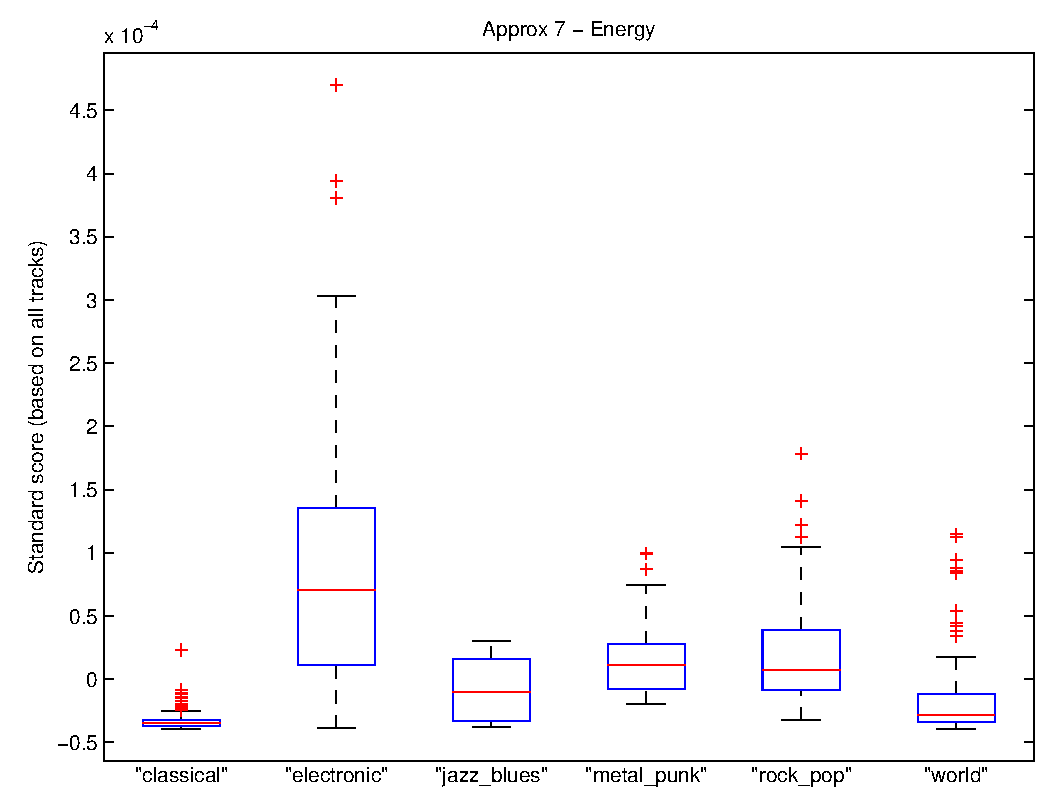
\includegraphics[width=0.45\textwidth]{figures/wch_box_08.pdf}
   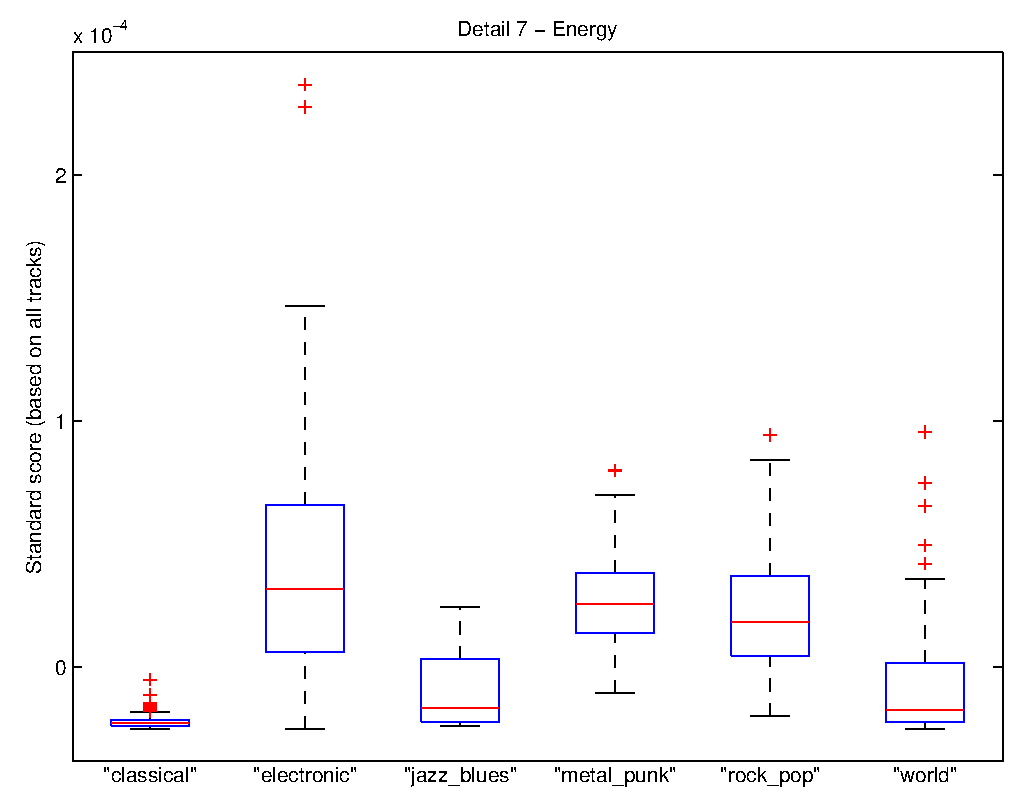
\includegraphics[width=0.45\textwidth]{figures/wch_box_16.pdf}
   \caption{Box plots of WCH energy from $7$th approximation and detail sub-band.}
   \label{fig:wch_box}
\end{figure}

\subsection{Creating a Feature Vector}
% TODO
\textbf{TODO}\\
We concatenate various features to make a feature vector for each song.  Explain which features we use.  Each feature (stored as a double, which may be overkill) will cost about 

\[ \dfrac{8}{1024^3}5\times10^8 \approx 3.7\,\text{GB} \] 

\noindent for every song ever created (about $500$ million).  We would certainly have fewer songs in our training DB, so the above size is a wild over estimate.

\subsection{Using Features for Distances}

Once the features of the songs have been collected, a distance between songs can be defined.  As noted previously, the simple features derived from the (Mel) power spectrum can be compared using the standard Euclidean distance.  However, for more complicated features like the Mel cepstrum, more sophisticated measures need to be used.

\subsection{Spectral Similarity Measures}
% TODO prolly want to trim this down a bit.
We wish to compare directly the Mel power spectrum of two songs.  This can be done by taking the discrete cosine transform (DCT) of Mel power spectrum for each segment of the song.  We then keep a subset of the coefficients and call them the Mel frequency cepstral coefficients (MFCCs).  Note that this is also reducing the dimensionality of the problem.  Once the MFCCs are computed, they are summarized by clustering the frames.  Songs may be compared by comparing the cluster model.\\

One possible cluster model fits a single Gaussian with mean $\mu$ and a full (as opposed to diagonal) covariance matrix $\Sigma$.  Cluster models of this form can be compared using a symmetric Kullback-Leibler divergence:

\[ d_{KL}\left(\left(\mu_1,\Sigma_1\right),\left(\mu_2,\Sigma_2\right)\right) = \operatorname{tr}\left(\Sigma_1\Sigma_2^{-1}\right) + \operatorname{tr}\left(\Sigma_1^{-1}\Sigma_2\right) + \operatorname{tr}\left(\left(\Sigma_1+\Sigma_2\right)(\mu_1-\mu_2)(\mu_1-\mu_2)^T\right). \]

\noindent These distances will span over many orders of magnitude, so it is wise to rescale the distance to

\[ d = -e^{-\frac{1}{450}d_{KL}}, \]

\noindent where the factor $450$ is recommended by Pampalk \cite{pampalk:dissertation}.\\

It is natural to want to extend the single Gaussian cluster model to a full Gaussian mixture model (GMM).  Instead of a single Gaussian, we attempt to fit a convex combination of $M$ Gaussians.  This distribution takes the form

\[ p(x|\Theta) = \sum_{i=1}^M P_i \mathcal{N}(\mu_i, \Sigma_i), \]

\noindent where $\Theta = \{P_i,\mu_i,\Sigma_i\}$, $P_i\ge 0$, $\sum_{i=1}^M P_i = 1$, and $\mu_i$ and $\Sigma_i$ are the mean and covariance of the $i$th Gaussian.  We wish to find the parameters in $\Theta$ that maximize the likelihood that that the frames $X = \{x_1,...,x_N\}$ were generated by the GMM with parameters $\Theta$.  The standard measure of likelihood is the log-likelihood

\[ L(X|\Theta) = \sum_{n=1}^N \log\left(p(x_n|\Theta)\right). \]

\noindent We can approach finding the optimal parameters $\Theta$ by using the expectation maximization algorithm, which is iterative and can be initialized using random initial data or an initial cluster given by $k$-means.  Two cluster models can be compared via log-likelihoods, giving the distance

\[ d = L(X_1|\Theta_1) + L(X_2|\Theta_2) - L(X_1|\Theta_2) - L(X_2|\Theta_1). \]

One may expect that a full GMM will provide better clustering than a single Gaussian, and thus a more accurate spectral similarity measure, but a working with full GMMs can become prohibitively expensive.  At the time of writing, we have implemented only the single Gaussian cluster model, which is much faster than a full GMM.\\

\subsubsection{Combining Distances}

Once we have chosen a spectral similarity measure and computed various simple features from the (Mel) power spectrum (e.g. median fluctuation patterns with Euclidean distance, center of gravity of fluctuation patterns with absolute value, etc.), we should combine the distances in a meaningful way.  One option is to use a convex combination of the $z$ (standard) scores of the distances.  This method gives the combined distance

\[ d = \sum_{i} w_i \left(\dfrac{d_i - \mu_i}{\sigma_i}\right) + \text{offset}, \]

\noindent where $w_i\ge 0$, $\sum_i w_i=1$, $d_i$ is the $i$th distance to be combined, $\mu_i$ and $\sigma_i$ are the mean and standard deviation of the $i$th distance over some reference set of songs (e.g. the entire database of songs), and the offset is chosen to the distance is positive for each pair of songs.  Pampalk describes a few possible combinations in his dissertation \cite{pampalk:dissertation}; we have implemented one and describe it below.\\


%_________________________________________________________________
\section{Dimension reduction}
%
%Describe your dimension reduction technique, and justify why it 
%is appropriate to use it in this context. You should explain what 
%performance is expected.
%_________________________________________________________________
% TODO Does he want us to justify the techniques we described above?

%One of the biggest challenges in data analysis is dealing with high dimensional data, both because of increased complexity in algorithms, and in interpreting high dimensional spaces.  Dimension reduction thus becomes important to bring the data into a space that is more manageable.\\
%
%In the context of music classification, much of the dimension reduction is done in the feature extraction stages.  A 3 minute song sampled at 44,100Hz (which is a standard sampling rate, but higher than we are dealing with in this project) is essentially a 7,938,000 dimensional vector.  Trying to compare multiple songs with this length vector is computationally expensive.  On top of that, the song does not actually live in a 7,938,000 dimensional space.  It likely lives in a much lower dimensional manifold.  The process of feature extraction which was discussed in the previous section is a big part of trying to describe songs in a lower dimensional space.\\
%
%Even after features are extracted from the songs, the space may be larger than desired.  For example, the Mel Frequency Cepstrum Coefficients for each song only reduce the dimension of the space by about one half.  For this reason, Gaussian approximations are applied to these Cepstrum coefficients, again as discussed in the previous section.  After all of the features are extracted and put into a more manageable form.  There could still be 30-60 features describing each song, with strong correlations between some of the features.\\
%
%At the post-feature extraction phase, the goal is to choose the features that best describe the songs, with a possibly different set of features for each genre, without overfitting.  PCA techniques can be applied to approximate the dimension of the space required to represent each genre, after which a search technique can be used to choose the best features.  Pompak \cite{pampalk:dissertation} discusses methods for choosing 2 or 7 features along with a spectral similarity measure to represent the song space, while Tzanetakis and Cook \cite{tzanetakis:classification} uses a 30 feature space, and Carlos et al. \cite{silla:selection} use a genetic algorithm based feature selection.

%_________________________________________________________________
\section{Statistical learning}
%Explain how the training data help find the genre of an unknown
%song. This could be as simple as finding the closest song among all
%the songs for which you know the genre. Or it could involve more
%sophisticated methods.
%_________________________________________________________________
\subsection{$K$-Nearest Neighbor}
One way to classify an observation is to use $K$-Nearest Neighbors. It is a simple machine learning algorithm that stores all the similarity measures of the training data and classifies a new observation based on the ``distance" of the testing data to the training data. It finds the  $K$ nearest neighbors and uses those observation to classify based on a majority vote. 

\subsection{Support Vector Machines}
Support vector machines is another simple machine learning algorithm. It defines each observation of the training data as a point in space and creates a boundary line that best separates the data into its correct classification with minimal amount of incorrect classifications. It then takes the testing data projects in down into the space and classifies the observation based on its relation to the boundary line. We can repeat this process until we have as many boundary lines as needed. To transform the boundary lines into a nonlinear form we can use kernel support vector machines.

\subsection{Cross-Validation}


To validate our classification algorithm, we want to use cross-validation which is a way for us to asses our results if were were to generalize to a new and independent data set. We want to get an idea about how well we are able to predict the genre correctly using a random subset of our training data as the test data since we are have the ground truth. Cross-validation also give us insight in the training phase of our algorithm to determine if we are over fitting. Overfitting the data occurs when the algorithm is predicting the error instead of true trends in the data. This can occur due to many factors, one of which is due to using too many features to describe the model, thus cross-validation can also inform which features or methods provide the best and consistent results. For our purpose we are using a leave-$p$-out-cross-validation method. This consists of leaving out $p$ observations of our training set and using the rest of the observations as our training data. We then repeat with all the different ways to cut the original data and compute the mean and the standard deviation of our results.

%_________________________________________________________________
\section{Experiments}
%Describe the experiments, and include the confusion matrix. Discuss
%the influence of the various parameters, and describe how the optimal
%parameters were chosen. Include the computation time for your method.
%_________________________________________________________________


%_________________________________________________________________
\section{Discussion}
%Provide a critique of the approach and discuss any potential
%improvement. Discuss the ability of your approach to classify
%non-classical into the five remaining genres.
%_________________________________________________________________


Dr. Meyer and James talked about wavelet stuff.  We should acknowledge his help in our conclusion.

% References
\bibliographystyle{siam}
\bibliography{mir}

\end{document}
